\documentclass[12pt]{article}
\linespread{1.25}
\usepackage{times}

\usepackage{pgfplots}
\pgfplotsset{compat = newest}
\usetikzlibrary{positioning, arrows.meta}
\usepgfplotslibrary{fillbetween}
\usepackage{amsmath}

\begin{document}

\begin{center}
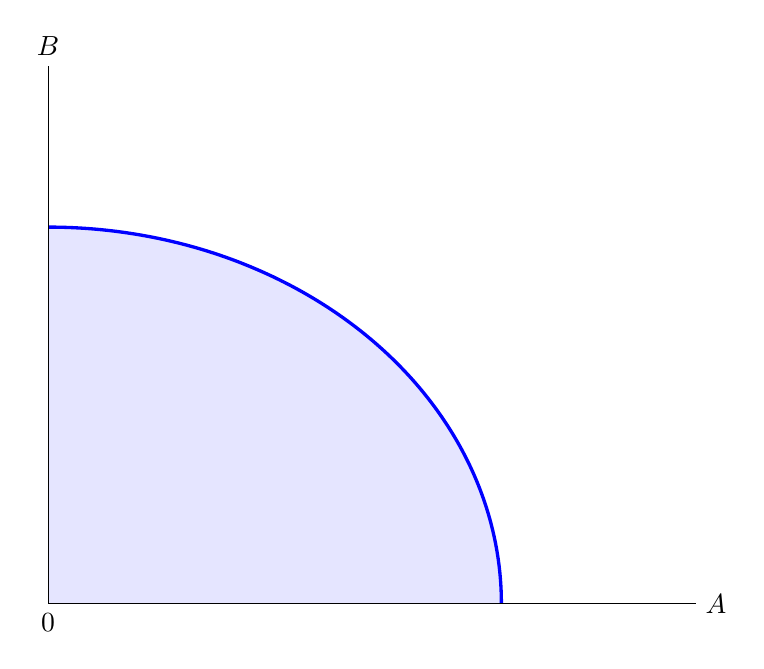
\begin{tikzpicture}
\begin{axis}[
scale = 1.2,
xmin = 0, xmax = 10,
ymin = 0, ymax = 10,
axis lines* = left,
xtick = {0}, ytick = \empty,
axis on top,
clip = false,
]
% Production-possibility frontier
\addplot [domain = 0:10, restrict y to domain = 0:10, samples=10000, color = blue, very thick, name path = frontier]{(49-x^2)^0.5};
\addplot [domain = 0:10, restrict y to domain = 0:10, draw = none, name path = axis]{0};

% Colouring areas
\addplot [blue,  opacity = 0.1] fill between [of = frontier and axis];

% Labels
\node [right] at (current axis.right of origin) {$A$};
\node [above] at (current axis.above origin) {$B$};
\end{axis}
\end{tikzpicture}
\end{center}
\textbf{Figure 5-9:} A production-possibility frontier between A and B.

\end{document}